
\chapter{系统实现}
\label{chap:achieve}

上文介绍了本系统的系统架构和逻辑功能。本章我们将进行部分的系统功能实现。由于本系统结构庞大,功能复杂,涉及许多不同体系的技术,所以限于篇幅有限,我们并不打算把系统涉及到的全部实现细节一一介绍。而只介绍其中最核心的,和最具有代表性的部分。

由于基于\smarkdown的文档撰写是本系统区别其他网络文档管理平台的最大特点。而且由于\smarkdown语法是本文作者在Markdown语法基础上扩展而来。所以介绍\smarkdown语法和它如何被渲染展示和如何被转换成\LaTeX,再进一步转换成最终的PDF文档将是我们本章介绍的重点。

由于Restful api是本系统的核心架构,所以api的实现也将是本章重点介绍的内容。

但是在介绍这两个部分之前,我们还是先来了解一下本系统主要涉及的技术,以及用到的编程语言,框架,和组件。

\section{系统涉及的实现技术}
\label{sec:language}

本系统要实现的功能繁多,而且要运行的平台也多样\footnote{windows应用,ios app,andriod app,web应用等}。最粗略的统计,主要包括:web service服务端、数据库、web前端、windows客户端和移动客户端几个部分。下面分别进行介绍:

\subsection{web service服务端}
\label{sec:webservice}

上文介绍过,本系统基本架构为restful的web服务。目前支持restful的编程语言和成型的开源架构很多,比如ROR、Python、java、.net等等。本系统选择的后端开发框架为Ruby on Rails,官方简称Rails,非RoR。它是使用Ruby脚本语言\footnote{一种为简单快捷面向对象编程而创的脚本语言,在20世纪90年代由日本人松本行弘开发。}所开发的Web开发框架。Rails是一套专业的开发框架,采用了MVC(Model-View-Control)模式、原生支持单元测试和整体测试、支持Ajax和RESTful结构、ORM机制,以及支持各种最新的业界标准像是HTML5、JQuery等等功能。它的发明人是David Heinemeier Hanson(DHH),DHH是2004年将Rails从37signals商业产品中独立出来的开源项目。它的设计目标是只要开发者熟悉它的惯例,就可以快速的开发网站。相比其他的语言和框架,Rails可以让你用更少的编码实现更多的功能。

选择Ruby on Rails的重要原因是:
\begin{itemize}
\item 它对RESTful的支持较好。可以说是原生支持,不用做任何配置就可以构建RESTful的web。
\item 支持多种格式的信息返回,一个后台服务可以支持web段程序,也可以提供api给其他客户端程序使用。
\item 采用它后生产力的暴增,写的的应用程序,增加新的功能都很容易。可以用更少的程序做更多的事情,而且程序维护起来更加容易。
\end{itemize}

当然Rails只是后台服务的基础架构,要完成本系统的诸多负载功能,还需要利用许多开源组件。

\subsection{数据库}
\label{sec:database}

本系统在数据库的使用上与传统的信息管理系统不同,我们将使用传统关系型数据库和非关系型数据库(nosql)相结合的方法。关系型数据库我们将使用开源的数据库mysql。关于这个数据库这里不过多的介绍,它是目前业界最常使用的开源关系型数据库系统。关于nosql,下面简单的做一个介绍。

nosql的主要特点包括非关系型、分布式、开源、水平可扩展。第一次看到这个名字,很多人都会认为nosql是“no sql”的简写,所以认为它是sql数据库的替代品,但实际上它是“not only sql”的简写,意思是不止用sql。它的出现主要是弥补关系型数据库的诸多缺点和不足:
\begin{enumerate}
\item 不擅长处理大量数据并发写入的应用。这也是近年来对关系型数据库的最大的诟病,因为通过增加硬件规模和性能来提高数据库读性能,但是由于数据一致性问题想提高写入性能会非常麻烦。进入web2.0时代,关系型数据库应对大量的SNS类型的动态网站时已经显得力不从心。
\item 不擅长处理字段不固定的应用。如果字段不固定,使用关系型数据库非常麻烦,尤其是目前主流的开发框架都使用数据库映射功能(ORM),如果字段不固定,那么开发的难度将非常大。
\end{enumerate}
而nosql数据库则可以很好的解决以上的问题:
\begin{enumerate}
\item nosql易于数据分散,可以通过简单的横向扩展来提高系统性能,而且读写性能均可以通过增加硬件规模和性能来得到线性的提升。
\item nosql可以轻松应对字段不固定的应用。
\end{enumerate}
通过第三章的介绍,我们知道,我们的系统既是一个高并发写入的SNS类的应用,同时也是一个字段不固定的应用。所以同时使用关系型数据库和nosql将很好的解决系统数据存储的问题。


目前常用的nosql数据库大致分为四种:
\begin{enumerate}
\item Key-value stores键值存储, memcached、Tokyo Tyrant、Redis等数据库属于这种类型。
\item Table-oriented 面向表, 主要代表有Google的BigTable和Cassandra。
\item Document-oriented面向文档,最常用的MongoDB 和 CouchDB。
\item Graph-oriented 面向图论, 如Neo4J。
\end{enumerate}
我们系统主要是用的是MongoDB这个面向文档的数据库。一方面,它是目前业界最广泛使用的nosql数据库。另外一方面,它面向文档的数据结构可以不用第一表结构,也支持复杂的查询条件,比较吻合本系统的需求。

\subsection{WEB前端}
\label{sec:webui}

对于最终用户,直接面对系统的就是用户界面(UI)。所以系统UI的好坏直接影响系统用户体验。本系统最先实现的也是最主要的用户界面就是WEB端的用户界面,也就是网页版的UI。虽然这么说并不准确,因为现在的WEB已经和几年前的网页大不相同了。WEB技术在近今年发展迅速,从一开始HTML的静态页面和applet小程序,到后来AJAX的流行,再到后来使用FLASH技术的富户端,甚至近两年炒的火热的HTML5。WEB技术的发展速度之快,让所有的WEB开发者叫苦不断,因为永远要学习新的技术。

本系统要使用的WEB前端框架叫做BootStrap,它是2011年twitter\footnote{最早也是世界上最流行的微博系统,被中国网墙屏蔽。}的“一小撮”工程师为了提高他们内部的分析和管理能力,用业余时间为他们的产品构建了一套易用、优雅、灵活、可扩展的前端工具集。Bootstrap由MARK OTTO和Jacob Thornton所设计和建立,在github上开源之后,迅速成为该站上最多人watch和fork的项目。大量工程师踊跃为该项目贡献代码,社区惊人地活跃,代码版本进化非常快速,官方文档质量极其高(可以说是优雅),同时涌现了许多基于Bootstrap建设的网站:界面清新、简洁;要素排版利落大方,如图~\ref{fig:xfig14}所示。

其次,系统门户界面可以使用Jekyll的模板系统,用户可以选择自己门户界面的模板。有兴趣的用户甚至可以自己编写门户模板提供给系统使用。

\begin{figure}[H]
  \centering
  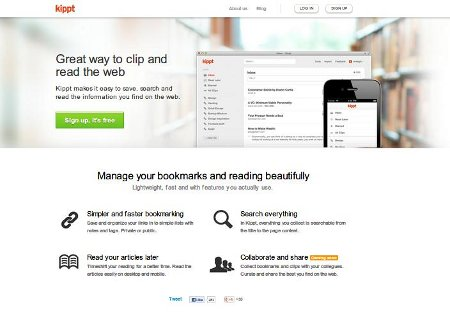
\includegraphics{bootstrap}
  \caption{Bootstrap界面}
  \label{fig:xfig14}
\end{figure}

\subsection{pc客户端和移动客户端}
\label{sec:pcandriodmac}

各种本地客户端程序可以通过标准的RESTful api访问系统数据。任何组织和个人在经过许可的情况下都可以开发并发布本系统的客户端程序。除此以外,我们也会提供官方的客户端程序。根据用户操作习惯的不同那个可以选择WEB方式或者本地客户端形式访问系统。下面简单介绍一下各种本地程序所使用的技术:
\begin{description}
\item[windows客户端] 主要采用c\#语言配合客户端界面的控件实现。
\item[Linux客户端] 使用C++和qt用户界面库实现。
\item[Mac客户端] 使用object c和cocoa开发框架实现。
\item[andriod客户端] 使用java和android开发套件实现。
\item[IOS客户端] 使用object c和Cocoa Touch框架实现。
\end{description}

除以上介绍的语言与框架外,任何编程语言与开发框架都可以用来开发本系统的本地客户端程序。

\section{\smarkdown语法}
\label{sec:smarkdownsyntax}

\smarkdown是以markdown语法为基础,并增加了学术文档中常用的表格、脚注、参考文献、代码块、属性列表、目录等语法内容,并且可以添加\LaTeX语法片段和文章属性字段。文章属性字段通过Liquid模板语言嵌入到文档中,并通过预处理机制替换成实际的内容。然后把替换后的文本交由\smarkdown引擎处理成xhtml格式进行显示。下面就分markdown基础语法、smarkdown扩展语法、嵌入属性语法、嵌入\LaTeX语法几个部分分别进行介绍。

\subsection{markdown基础语法}
\label{sec:markdownbase}

\begin{description}
\item[段落] 一个段落是由一个以上的连接的行句组成,而一个以上的空行则会划分出不同的段落(空行的定义是显示上看起来像是空行,就被视为空行,例如有一行只有空白和 tab,那该行也会被视为空行),一般的段落不需要用空白或换行缩进。
\item[标题] Markdown 支持两种标题的语法,Setext 和 atx 形式。Setext 形式是用底线的形式,利用 = (最高阶标题)和 - (第二阶标题),Atx 形式在行首插入 1 到 6 个 \# ,对应到标题 1 到 6 阶。
\item[区块代码] 区块引用使用 email 形式的 '>' 角括号。
\item[强调] Markdown 使用星号和底线来标记需要强调的区段。比如:*强调*、\_强调\_、**强调** 都表示加粗显示。
\item[无序列表] 无序列表使用星号、加号和减号来做为列表的项目标记,这些符号是都可以使用。
\item[有序列表] 有序的列表则是使用一般的数字接着一个英文句点作为项目标记。
\item[链接] Markdown 支援两种形式的链接语法: 行内 和 参考 两种形式,两种都是使用角括号来把文字转成连结。行内形式是直接在后面用括号直接接上链接,参考形式的链接让你可以为链接定一个名称,之后你可以在文件的其他地方定义该链接的内容。
\item[图片] 图片的语法和链接很像,只不过把链接的地址换成图片的地址。本系统中,用户要向文档添加图片非常方便,可以直接填写网络图片库的图片地址,也可以从本机上传图片,上传后系统将自动为用户填写好Markdown的图片语法。
\item[嵌入HTML] 在一般的段落文字中,你可以使用反引号 ` 来标记代码区段,区段内的 \&、< 和 > 都会被自动的转换成 HTML 实体,这项特性让你可以很容易的在代码区段内插入 HTML 码。
\end{description}
虽然Markdown语法简单易学,而且在网络时代非常流行,被越来越多的网络编辑系统所采用,但是它只定义了网络媒体中常用的表达方式,用来书写科技文档还略显不足。所以本系统在Markdown基础语法的基础上对其进行了扩展,以满足书写科技文档常用的格式需求。

\subsection{\smarkdown扩展语法}
\label{sec:smarkdownextr}

\begin{description}
\item[表格] 如下例子所示,表格第一行包含列标题,第二行包含位于标题和内容之间的强制性分隔线,接下来的每一行就是表格的内容。列与列之间用竖线 | 分隔。如果愿意的话,可以在表格每一行的开头和结尾处添加竖线 |。输出的结果一样。通过在对应列的分隔线添加冒号 : 可以指定列的对齐方式。冒号 : 在分隔线的左边说明此列左对齐,冒号 : 在分隔线的右边说明此列右对齐,冒号 : 在分隔线的左右两边说明此列居中。
  \begin{bframe}
    Col1     |                  标题                   |               标题                  |\\
    - - - - -|:- - - - - - - - - - - - - - - - - - - :|- - - - - - - - - - - - - - - - - -:|\\
    cell     |                中间对齐                 |              右对齐                 |\\
  \end{bframe}
\item[脚注] 脚注是在需要标记脚注文字的后面增加一个方括号,方括号中的内容必须以  \^{} 开头,再接着是数字、字符串标记,接着,在文件的任意地方,你可以把这个脚注的内容定义出来.例如:
  \begin{bframe}
    Footnotes[\^{} 1] have a label[ \^{}label] and a definition[\^{}!DEF]\\
    %[\^{} 1] This is a footnote
    %[\^{}label]: A footnote on "label"\\
    %[\^{}!DEF]: The definition of a footnote.\\
  \end{bframe}
\item[高亮代码块] 使用反引号,加语言名。支持多种语言,比如 python, c, html 等,。
  \begin{bframe}
    ```python\\
   def hello():\\
    return 'Hello World'\\
    ```\\
  \end{bframe}
\item[属性列表] 定义 HTML 元素的属性。可以自定义文本内容的id和css类。
\item[目录] 在需要目录出现的地方放置一个标记,这样会自动生成一个嵌套的包含所有标题的列表。默认的标记是 [TOC]。目录跳转的标题 id 是依据标题内容自动生成的,只包含英文、数字、下划线 \_ 等。对于全部是中文的标题,自动生成的标题 id 为空,导致无法跳转。可以使用属性列表方法,定义标题 id。
\end{description}
\subsection{嵌入属性语法}
\label{sec:addattr}

前文提到,任何一个文档都可以定义若干属性,在文档中可以添加这些属性。由于属性有多种类型,每种类型的表现形式也不近相同。所以系统为每一种属性都提供了若干表现方式可以供文档显示,比如:一个数字属性叫做aint,那么如果要显示该数字,并只保留两位小数,可以使用数字类型的format样式函数输出。每种类型的属性支持的样式函数不同,比如,一个pdf类型的文档就支持pagenum(页数)函数,和cutpage(取前多少页)函数。

属性插入文档的语法按照Liquid模板引擎语言设计,插入时直接用\{\{属性名.样式函数\}\}这样的结构加入到文档中,文档在被翻译成其他格式前,先进行预处理,把属性替换成显示的样子和文档一起显示。

\subsection{\LaTeX片段语法}
\label{sec:latexpic}

对于一般的科技文档撰写,系统提供的\smarkdown语法已经基本上可以满足大部分用户的需求了。但是为了满足有些数学和力学专业的用户,本系统还提供了在\smarkdown文档中直接添加\LaTeX数学公式片段的功能\footnote{由于\LaTeX片段只有在把文档转换成\LaTeX文档的时候才会编译,所以文档包含的\LaTeX片段在预览和WEB显示时无法显示完整的输出格式。}。

\LaTeX数学片段的语法很简单,直接把行内\LaTeX数学公式源代码写到文档中以\$为标志的区间内就可以。区间内的公式片段将保留到\LaTeX编译阶段直接输出公式。而将独立公式放入以\$\$.....\$\$或者[.....]的区块中就可以。
